\documentclass[12pt, a4paper]{book}
\begin{document}
While the standard model of particle physics has been incredibly successful in describing the behavior of subatomic particles, it is not a complete description of the universe. For example, the standard model cannot accommodate the mysterious gravitational forces that hold galaxies together, 
and it fails to account for the abundance of matter that we observe in the universe.\\
\\These mysteries have led scientists to propose the existence of Dark Matter (DM), a mysterious substance that makes up a significant fraction of the matter in the universe. The name DM, stems from the understanding that while most DM particles do not interact with matter via any of the forces described by the SM. 
However, it is important to note that certain DM candidates can indeed interact weakly through the weak force as described by the SM. This makes it extremely difficult to detect directly. However, its presence can be inferred through its gravitational effects on visible matter, such as stars and galaxies, which is why we know it is there \cite{DM1, DM2}. In this thesis we will look at so-called 
Weakly Interacting Massive Particles (WIMP) DM candidates. There is no formal definition of a WIMP, but broadly it is a new elementary particle which interacts via gravity, possibly the weak interaction, and potentially other forces outside the SM.\\
\\There are several extensions of the SM that include DM candidate particles interacting via a so-called Beyond Standard Model (BSM) Lagrangian. Such as Supersymmetry \cite{JUNGMAN1996195},  Universal Extra Dimensions \cite{DIENES199947} and little Higgs models \cite{ARKANIHAMED2001232}. 
In this chapter we will present the BSM models we will be studying that have a dilepton and MET final state.

\section{Mono-Z' candidates}
Six of the models that will be studied in this thesis come from a new theoretical gauge boson that behaves like much heavier $Z$ boson. The theory is based on the papers by Bauer et al. \cite{ Zp_DM_candidate2}. % which have previously been studied by ATLAS \cite{Zp_DM_candidate3} and CMS collaborations \cite{Zp_DM_candidate1}. \\
The models we will study assume a $U(1)'$ symmetry for a new $Z'$ gauge boson, from this we can extend the SM Lagrangian, to include the $Z'$ coupling to the SM particles by
\begin{equation}\label{eq:Zpq}
    \mathcal{L}\supset -\sum_q g_q \overline{q}\gamma^\mu q Z'_\mu
\end{equation}
where the coupling $g_q$ is a free parameter of the model. The three models we will study are based on three interactions of this new $Z'$ (decaying into two leptons) and DM candidates $\chi$ which we describe now.
% which again are divided into a Heavy Dark Sector (HDS) and Light Dark Sector (LDS) based on the mass of the DM candidate, for more information on this and the selection of parameters see Chapter \ref{chap:DM_sample}.

\subsection{Z' Dark Higgs}
The DM $Z'$ models come with an additional scalar responsible for SSB. A new scalar particle that couples to the $Z'$, which we will call the Dark Higgs (DH), $h_D$, plays the role of portal to DM. Analogous to the SM process of Higgs-boson radiation from a $W$ or $Z$, the DH is radiated from the $Z'$ in a dark-Higgsstrahlung process. 
In addition, we will assume that this DH boson couples with invisible states, such as DM. A minimal model for this process, with the $U(1)'$ symmetry with a charged scalar field $\Phi_D$ as well as an invisible singlet scalar $\phi_\chi$:
\begin{equation}
    \mathcal{L}\supset \abs{D_\mu\Phi_D}^2 + \mu_D^2\abs{\Phi_D}^2 -\lambda_D\abs{\Phi_D}^2-\frac{1}{4}(F'_{\mu\nu})^2 + \frac{1}{2}(\partial_\mu\phi_\chi)-\lambda_\chi\abs{\Phi_D}^2\phi_\chi^2 - V(\phi_\chi)
\end{equation}
with $\Phi_D =\frac{1}{\sqrt{2}}(v_D+h_D)$, thus obtaining a vacuum expectation value giving mass to the $Z'$, $m_{Z'}$. The coupling of the DH with $Z'$ is
\begin{equation}
    Q_hg_Zm_{Z'}h_DZ'_\mu Z'^\mu \equiv g_{h_D}m_{Z'}h_DZ'_\mu Z'^\mu
\end{equation}
where $Q_h$ is the charge of the $\Phi_D$ which is a free parameter absorbed in the coupling $g_{h_D}$ above. The Feynman diagram for this dark Higgs model is depicted in Figure \ref{fig:DH}
\begin{figure}[!ht]
    \centering
    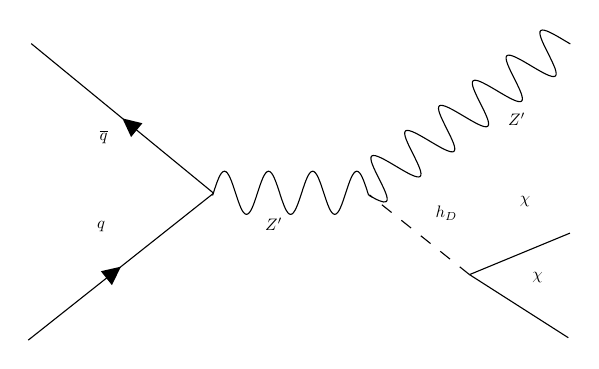
\begin{tikzpicture}[x=0.75pt,y=0.75pt,yscale=-1,xscale=1]
        %uncomment if require: \path (0,300); %set diagram left start at 0, and has height of 300
        
        %Straight Lines [id:da27662717418171545] 
        \draw    (287.31,132.97) -- (197.99,203.77) ;
        \draw [shift={(242.65,168.37)}, rotate = 141.6] [fill={rgb, 255:red, 0; green, 0; blue, 0 }  ][line width=0.08]  [draw opacity=0] (8.93,-4.29) -- (0,0) -- (8.93,4.29) -- cycle    ;
        %Straight Lines [id:da5113223214900172] 
        \draw    (199.42,60.88) -- (287.31,132.97) ;
        \draw [shift={(243.36,96.92)}, rotate = 39.36] [fill={rgb, 255:red, 0; green, 0; blue, 0 }  ][line width=0.08]  [draw opacity=0] (8.93,-4.29) -- (0,0) -- (8.93,4.29) -- cycle    ;
        %Shape: Wave [id:dp2919243358600071] 
        \draw   (362.02,133.92) .. controls (365.96,136.19) and (369.33,137.87) .. (370.5,137) .. controls (371.97,135.91) and (369.56,131.08) .. (367.01,126.02) .. controls (364.47,120.95) and (362.06,116.12) .. (363.53,115.03) .. controls (365,113.93) and (369.96,116.88) .. (375.15,119.97) .. controls (380.35,123.07) and (385.31,126.01) .. (386.78,124.92) .. controls (388.25,123.82) and (385.84,118.99) .. (383.3,113.93) .. controls (380.75,108.86) and (378.34,104.03) .. (379.81,102.94) .. controls (381.29,101.84) and (386.24,104.79) .. (391.44,107.88) .. controls (396.64,110.98) and (401.59,113.92) .. (403.06,112.83) .. controls (404.54,111.73) and (402.12,106.9) .. (399.58,101.84) .. controls (397.04,96.77) and (394.62,91.94) .. (396.1,90.85) .. controls (397.57,89.76) and (402.52,92.7) .. (407.72,95.79) .. controls (412.92,98.89) and (417.87,101.83) .. (419.35,100.74) .. controls (420.82,99.64) and (418.41,94.82) .. (415.86,89.75) .. controls (413.32,84.68) and (410.91,79.85) .. (412.38,78.76) .. controls (413.85,77.67) and (418.81,80.61) .. (424,83.7) .. controls (429.2,86.8) and (434.16,89.74) .. (435.63,88.65) .. controls (437.1,87.56) and (434.69,82.73) .. (432.15,77.66) .. controls (429.6,72.59) and (427.19,67.77) .. (428.66,66.67) .. controls (430.14,65.58) and (435.09,68.52) .. (440.29,71.62) .. controls (445.49,74.71) and (450.44,77.65) .. (451.91,76.56) .. controls (453.39,75.47) and (450.97,70.64) .. (448.43,65.57) .. controls (445.89,60.5) and (443.47,55.68) .. (444.95,54.58) .. controls (446.42,53.49) and (451.37,56.43) .. (456.57,59.53) .. controls (457.46,60.05) and (458.33,60.58) .. (459.19,61.07) ;
        %Shape: Wave [id:dp11315736537659926] 
        \draw   (286.79,134.08) .. controls (286.93,133.65) and (287.07,133.22) .. (287.21,132.78) .. controls (288.95,127.45) and (290.6,122.38) .. (292.53,122.38) .. controls (294.45,122.38) and (296.11,127.45) .. (297.84,132.78) .. controls (299.57,138.11) and (301.23,143.18) .. (303.16,143.18) .. controls (305.08,143.18) and (306.74,138.11) .. (308.47,132.78) .. controls (310.2,127.45) and (311.86,122.38) .. (313.78,122.38) .. controls (315.71,122.38) and (317.36,127.45) .. (319.1,132.78) .. controls (320.83,138.11) and (322.49,143.18) .. (324.41,143.18) .. controls (326.33,143.18) and (327.99,138.11) .. (329.73,132.78) .. controls (331.46,127.45) and (333.12,122.38) .. (335.04,122.38) .. controls (336.96,122.38) and (338.62,127.45) .. (340.35,132.78) .. controls (342.09,138.11) and (343.74,143.18) .. (345.67,143.18) .. controls (347.59,143.18) and (349.25,138.11) .. (350.98,132.78) .. controls (352.71,127.45) and (354.37,122.38) .. (356.3,122.38) .. controls (358.22,122.38) and (359.88,127.45) .. (361.61,132.78) .. controls (361.73,133.15) and (361.85,133.51) .. (361.97,133.88) ;
        %Straight Lines [id:da18657926730805996] 
        \draw  [dash pattern={on 4.5pt off 4.5pt}]  (410.6,172.2) -- (362.39,133.77) ;
        %Straight Lines [id:da4524964685792049] 
        \draw    (410.6,172.2) -- (459,152.2) ;
        %Straight Lines [id:da34778222034828554] 
        \draw    (458.2,202.6) -- (410.6,172.2) ;
        
        % Text Node
        \draw (230.38,145.99) node [anchor=north west][inner sep=0.75pt]  [xscale=0.6,yscale=0.6]  {$q$};
        % Text Node
        \draw (231.63,101.74) node [anchor=north west][inner sep=0.75pt]  [xscale=0.6,yscale=0.6]  {$\overline{q}$};
        % Text Node
        \draw (311.36,144.25) node [anchor=north west][inner sep=0.75pt]  [xscale=0.6,yscale=0.6]  {$Z'$};
        % Text Node
        \draw (393.47,138.4) node [anchor=north west][inner sep=0.75pt]  [xscale=0.6,yscale=0.6]  {$h_{D}$};
        % Text Node
        \draw (428.48,93.62) node [anchor=north west][inner sep=0.75pt]  [xscale=0.6,yscale=0.6]  {$Z'$};
        % Text Node
        \draw (434.16,133.87) node [anchor=north west][inner sep=0.75pt]  [xscale=0.6,yscale=0.6]  {$\chi $};
        % Text Node
        \draw (440.16,170.27) node [anchor=north west][inner sep=0.75pt]  [xscale=0.6,yscale=0.6]  {$\chi $};
        
        
        \end{tikzpicture}
    
    \caption{Z' Dark Higgs Model}\label{fig:DH}
\end{figure}

\subsection{Z' Light Vector}
The second mono-$Z'$ model we will look at, is when the $Z'$ is relatively light such that it can be produced in $q\overline{q}$ annihilation and decays to dark states. As an example we can consider a $Z'$ 
coupled to a new fermion which has both Dirac and Majorana masses, $M_d$ and $M_m$ respectively. Where the Majorana mass can be generated from the $U(1)'$ through a $y_\chi\Phi_\chi\overline{\chi}\chi^c$, such that
$$
\mathcal{L}\supset \overline{\chi}(i\slashed{D}-M_d)\chi - \frac{M_m}{2}(\overline{\chi}\chi + h.c)
$$
This leads to two Majorana states $\chi_{1,2}$ with masses $M_{1,2}=\abs{M_m\pm M_d}$. We will study the process $Z'\rightarrow\chi_1\chi_2$, where $\chi_2\rightarrow Z'\chi_1$. This model is represented in the Feynman diagram in Figure \ref{fig:LV}
\begin{figure}[!ht]
    \centering
    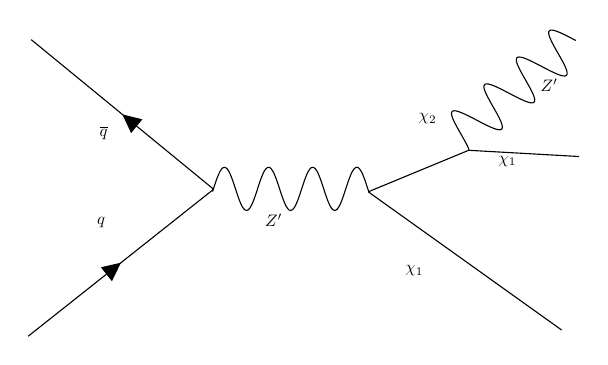
\begin{tikzpicture}[x=0.75pt,y=0.75pt,yscale=-1,xscale=1]
    %uncomment if require: \path (0,300); %set diagram left start at 0, and has height of 300

    %Straight Lines [id:da27662717418171545] 
    \draw    (287.31,132.97) -- (197.99,203.77) ;
    \draw [shift={(242.65,168.37)}, rotate = 141.6] [fill={rgb, 255:red, 0; green, 0; blue, 0 }  ][line width=0.08]  [draw opacity=0] (8.93,-4.29) -- (0,0) -- (8.93,4.29) -- cycle    ;
    %Straight Lines [id:da5113223214900172] 
    \draw    (199.42,60.88) -- (287.31,132.97) ;
    \draw [shift={(243.36,96.92)}, rotate = 39.36] [fill={rgb, 255:red, 0; green, 0; blue, 0 }  ][line width=0.08]  [draw opacity=0] (8.93,-4.29) -- (0,0) -- (8.93,4.29) -- cycle    ;
    %Shape: Wave [id:dp2919243358600071] 
    \draw   (410.48,114.25) .. controls (409.77,112.16) and (408.09,109.23) .. (406.37,106.2) .. controls (403.55,101.28) and (400.88,96.59) .. (402.29,95.42) .. controls (403.7,94.25) and (408.81,96.92) .. (414.17,99.73) .. controls (419.53,102.54) and (424.63,105.21) .. (426.04,104.04) .. controls (427.46,102.86) and (424.78,98.17) .. (421.97,93.25) .. controls (419.16,88.33) and (416.49,83.64) .. (417.9,82.47) .. controls (419.31,81.3) and (424.42,83.97) .. (429.77,86.78) .. controls (435.13,89.59) and (440.24,92.26) .. (441.65,91.08) .. controls (443.06,89.91) and (440.39,85.22) .. (437.58,80.3) .. controls (434.76,75.38) and (432.09,70.69) .. (433.5,69.52) .. controls (434.92,68.34) and (440.02,71.01) .. (445.38,73.82) .. controls (450.74,76.63) and (455.84,79.3) .. (457.26,78.13) .. controls (458.67,76.96) and (456,72.27) .. (453.18,67.35) .. controls (450.37,62.43) and (447.7,57.74) .. (449.11,56.56) .. controls (450.52,55.39) and (455.63,58.06) .. (460.99,60.87) .. controls (461.27,61.02) and (461.55,61.17) .. (461.83,61.32) ;
    %Shape: Wave [id:dp11315736537659926] 
    \draw   (286.79,134.08) .. controls (286.93,133.65) and (287.07,133.22) .. (287.21,132.78) .. controls (288.95,127.45) and (290.6,122.38) .. (292.53,122.38) .. controls (294.45,122.38) and (296.11,127.45) .. (297.84,132.78) .. controls (299.57,138.11) and (301.23,143.18) .. (303.16,143.18) .. controls (305.08,143.18) and (306.74,138.11) .. (308.47,132.78) .. controls (310.2,127.45) and (311.86,122.38) .. (313.78,122.38) .. controls (315.71,122.38) and (317.36,127.45) .. (319.1,132.78) .. controls (320.83,138.11) and (322.49,143.18) .. (324.41,143.18) .. controls (326.33,143.18) and (327.99,138.11) .. (329.73,132.78) .. controls (331.46,127.45) and (333.12,122.38) .. (335.04,122.38) .. controls (336.96,122.38) and (338.62,127.45) .. (340.35,132.78) .. controls (342.09,138.11) and (343.74,143.18) .. (345.67,143.18) .. controls (347.59,143.18) and (349.25,138.11) .. (350.98,132.78) .. controls (352.71,127.45) and (354.37,122.38) .. (356.3,122.38) .. controls (358.22,122.38) and (359.88,127.45) .. (361.61,132.78) .. controls (361.73,133.15) and (361.85,133.51) .. (361.97,133.88) ;
    %Straight Lines [id:da4524964685792049] 
    \draw    (361.8,134.2) -- (410.2,114.2) ;
    %Straight Lines [id:da34778222034828554] 
    \draw    (455,200.8) -- (361.8,134.2) ;
    %Straight Lines [id:da21909750853077148] 
    \draw    (410.2,114.2) -- (463.4,117.2) ;

    % Text Node
    \draw (230.38,145.99) node [anchor=north west][inner sep=0.75pt]  [xscale=0.6,yscale=0.6]  {$q$};
    % Text Node
    \draw (231.63,101.74) node [anchor=north west][inner sep=0.75pt]  [xscale=0.6,yscale=0.6]  {$\overline{q}$};
    % Text Node
    \draw (311.36,144.25) node [anchor=north west][inner sep=0.75pt]  [xscale=0.6,yscale=0.6]  {$Z'$};
    % Text Node
    \draw (444.08,79.22) node [anchor=north west][inner sep=0.75pt]  [xscale=0.6,yscale=0.6]  {$Z'$};
    % Text Node
    \draw (385.36,95.87) node [anchor=north west][inner sep=0.75pt]  [xscale=0.6,yscale=0.6]  {$\chi _{2}$};
    % Text Node
    \draw (378.96,169.07) node [anchor=north west][inner sep=0.75pt]  [xscale=0.6,yscale=0.6]  {$\chi _{1}$};
    % Text Node
    \draw (423.76,116.27) node [anchor=north west][inner sep=0.75pt]  [xscale=0.6,yscale=0.6]  {$\chi _{1}$};


    \end{tikzpicture}
    \caption{Z' Light Vector Model}\label{fig:LV}
\end{figure}
\\It is assumed that the mass splitting of the two states, $\chi_{1,2}$, is larger than $m_{Z'}$, such that the heavier state, $\chi_2$ can decay into an on-shell $Z'$ and a stable DM candidate $\chi_1$. The $\chi_{1,2}$ interaction with the $Z'$ is off-diagonal,
and taking $M_m>M_d$ we can write the interaction
\begin{equation}
    \frac{g_\chi}{2}Z'_\mu(\overline{\chi}_2\gamma^\mu\gamma^5\chi_1 + \overline{\chi}_1\gamma^\mu\gamma^5\chi_2)
\end{equation}

\subsection{Z' Effective Field Theory}
The aforementioned models rely on the $Z'$ coupling to the quarks as seen in Eq. (\ref{eq:Zpq}). In the third model, rather than producing the DM candidates through the new $Z'$, 
we consider the possibility that the dark states $\chi_1$ and $\chi_2$ are produced through a new constant interaction: 
\begin{equation}\label{eq:EFT_DM}
    \frac{1}{2\Lambda^2}\overline{q}\gamma_\mu q(\overline{\chi}_2\gamma^\mu\gamma^5\chi_1 + \overline{\chi}_1\gamma^\mu\gamma^5\chi_2),
\end{equation}
where $\Lambda$ is the scale at which new physics may appear. Similarly to the Light Vector model we assume the two dark states $\chi_{1,2}$ with an off-diagonal coupling to the $Z'$, however, the intermediate $s$-channel $Z'$ in Figure \ref{fig:LV} has effectively 
been replaced with a heavy $Z'_H$, which has been integrated out to give the operator in Eq. (\ref{eq:EFT_DM}). This results in the process of in Figure \ref{fig:EFT}.
\begin{figure}[!ht]
    \centering
    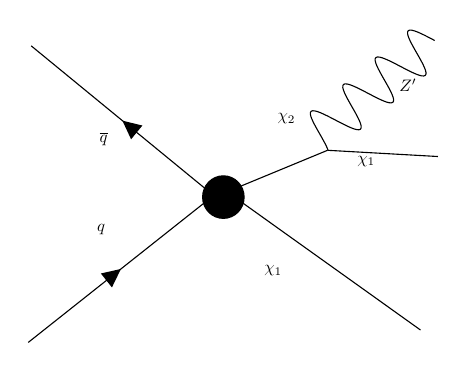
\begin{tikzpicture}[x=0.75pt,y=0.75pt,yscale=-1,xscale=1]
        %uncomment if require: \path (0,300); %set diagram left start at 0, and has height of 300
        
        %Straight Lines [id:da27662717418171545] 
        \draw    (324.81,138.97) -- (235.49,209.77) ;
        \draw [shift={(280.15,174.37)}, rotate = 141.6] [fill={rgb, 255:red, 0; green, 0; blue, 0 }  ][line width=0.08]  [draw opacity=0] (8.93,-4.29) -- (0,0) -- (8.93,4.29) -- cycle    ;
        %Straight Lines [id:da5113223214900172] 
        \draw    (236.92,66.88) -- (324.81,138.97) ;
        \draw [shift={(280.86,102.92)}, rotate = 39.36] [fill={rgb, 255:red, 0; green, 0; blue, 0 }  ][line width=0.08]  [draw opacity=0] (8.93,-4.29) -- (0,0) -- (8.93,4.29) -- cycle    ;
        %Shape: Wave [id:dp2919243358600071] 
        \draw   (379.98,117.25) .. controls (379.27,115.16) and (377.59,112.23) .. (375.87,109.2) .. controls (373.05,104.28) and (370.38,99.59) .. (371.79,98.42) .. controls (373.2,97.25) and (378.31,99.92) .. (383.67,102.73) .. controls (389.03,105.54) and (394.13,108.21) .. (395.54,107.04) .. controls (396.96,105.86) and (394.28,101.17) .. (391.47,96.25) .. controls (388.66,91.33) and (385.99,86.64) .. (387.4,85.47) .. controls (388.81,84.3) and (393.92,86.97) .. (399.27,89.78) .. controls (404.63,92.59) and (409.74,95.26) .. (411.15,94.08) .. controls (412.56,92.91) and (409.89,88.22) .. (407.08,83.3) .. controls (404.26,78.38) and (401.59,73.69) .. (403,72.52) .. controls (404.42,71.34) and (409.52,74.01) .. (414.88,76.82) .. controls (420.24,79.63) and (425.34,82.3) .. (426.76,81.13) .. controls (428.17,79.96) and (425.5,75.27) .. (422.68,70.35) .. controls (419.87,65.43) and (417.2,60.74) .. (418.61,59.56) .. controls (420.02,58.39) and (425.13,61.06) .. (430.49,63.87) .. controls (430.77,64.02) and (431.05,64.17) .. (431.33,64.32) ;
        %Straight Lines [id:da4524964685792049] 
        \draw    (331.3,137.2) -- (379.7,117.2) ;
        %Straight Lines [id:da34778222034828554] 
        \draw    (424.5,203.8) -- (331.3,137.2) ;
        %Straight Lines [id:da21909750853077148] 
        \draw    (379.7,117.2) -- (432.9,120.2) ;
        %Flowchart: Connector [id:dp3106597870190554] 
        \draw  [fill={rgb, 255:red, 0; green, 0; blue, 0 }  ,fill opacity=1 ] (319.5,139.75) .. controls (319.5,134.09) and (323.98,129.5) .. (329.5,129.5) .. controls (335.02,129.5) and (339.5,134.09) .. (339.5,139.75) .. controls (339.5,145.41) and (335.02,150) .. (329.5,150) .. controls (323.98,150) and (319.5,145.41) .. (319.5,139.75) -- cycle ;
        
        % Text Node
        \draw (267.88,151.99) node [anchor=north west][inner sep=0.75pt]  [xscale=0.6,yscale=0.6]  {$q$};
        % Text Node
        \draw (269.13,107.74) node [anchor=north west][inner sep=0.75pt]  [xscale=0.6,yscale=0.6]  {$\overline{q}$};
        % Text Node
        \draw (413.58,82.22) node [anchor=north west][inner sep=0.75pt]  [xscale=0.6,yscale=0.6]  {$Z'$};
        % Text Node
        \draw (354.86,98.87) node [anchor=north west][inner sep=0.75pt]  [xscale=0.6,yscale=0.6]  {$\chi _{2}$};
        % Text Node
        \draw (348.46,172.07) node [anchor=north west][inner sep=0.75pt]  [xscale=0.6,yscale=0.6]  {$\chi _{1}$};
        % Text Node
        \draw (393.26,119.27) node [anchor=north west][inner sep=0.75pt]  [xscale=0.6,yscale=0.6]  {$\chi _{1}$};
        
        
    \end{tikzpicture}
    \caption{Z' Effective Field Theory Model}\label{fig:EFT}
\end{figure}

\newpage
\section{Supersymmetry}
Supersymmetry, or SUSY for short, is another SM extension that introduces a new symmetry between fermions and bosons. A supersymmetrical operator, $Q$, changes a particle from a fermionic state, $\ket{F}$, to a bosonic state, $\ket{B}$, 
and vice versa by changing the spin by 1/2 unit 
$$
Q\ket{F} = \ket{B},\quad\text{and}\quad Q\ket{B} = \ket{F}
$$
This new symmetry has as a consequence that for each fermion degree of freedom in the SM, 
there must be a boson degree of freedom and vice versa. What this means is that every SM particle has a superpartner, such that SM particles are grouped with their supersymmetric counterpart into supermultiplets according to their quantum numbers.\footnote{The supersymmetric operator, $Q$, does not change any of the quantum numbers except for the spin }\\
\\This extension addresses many of the problems in the SM, but for the purposes of this thesis we will only mention the \textit{WIMP miracle} \cite{JUNGMAN1996195}. 
To give a brief description of the WIMP miracle, if we put in the dark matter density that the universe requires today, we can infer how many WIMPs\footnote{Assuming they interact only through the weak force and gravity} we need of a given mass to make it up. 
With this we can compute what the self-annihilation cross-section must be in order to get the right abundance of dark matter in the universe.
That value turns out to be in the range of the electroweak scale. For SUSY the DM mass scale is in the ballpark of 100 GeV to 1 TeV, suggesting that the self-annihilation of SUSY WIMPs in the early universe could have naturally resulted in the observed dark matter abundance we see today. 
During the cooling of the universe, the self-annihilation of WIMPs eventually stopped, known as freeze-out. This freeze-out process led to a constant population of WIMPs, preserving a certain relic density. This relic density is suggested to be what we observe today as dark matter, indicating the importance of freeze-out in determining the abundance of dark matter particles in the universe.\\
\\The neutralino, $\tilde{\chi}_1^0$, is a leading candidate for dark matter because it naturally emerges as the lightest supersymmetric particle, and is in the SUSY models studied in this thesis assumed to be typically stable. As a WIMP, the neutralino possesses the appropriate properties to be a dark matter candidate, 
interacting weakly with other particles and having a mass scale consistent with the observed dark matter density in the universe. Because of this we will look at a model which has neutralinos in the final state. The model we will study, 
which has been studied by the ATLAS collaboration \cite{ATLAS:2022hbt}, is the \textit{direct slepton production} channel as this has a dilepton and MET final state, which this thesis is based on.\\
\\For this thesis we will study a process involving superpartners of the leptons, the sleptons, $\tilde{\ell}$, as illustrated in the Feynman diagram in Figure \ref{fig:SlepSlep}.
\graphicspath{{../../figures/}}
\begin{figure}[!ht]
    \centering
    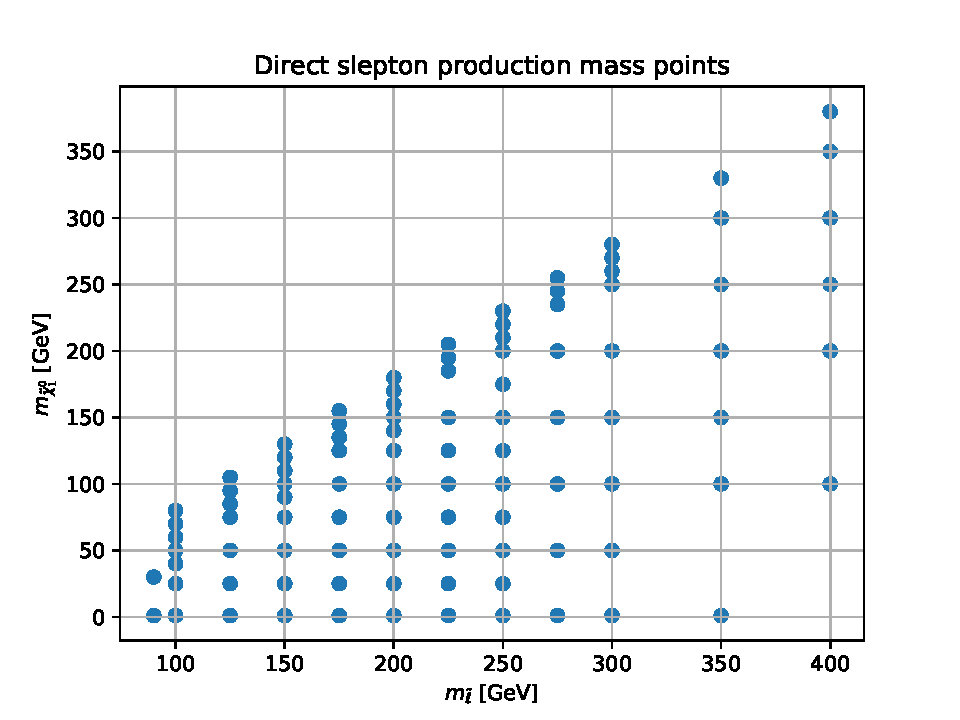
\includegraphics[width=0.4\textwidth]{SlepSlep.png}
    \caption{Supersymmetric direct slepton production model}\label{fig:SlepSlep}
\end{figure}
\\In this model we study sleptons produced in the $pp-$collisions at the LHC, which then decay to their SM partner, the leptons, in addition to the DM candidate the neutralino, $\tilde{\chi}_1^0$. In this thesis only the 1st and 2nd generation\footnote{The superymmetric partners of the electron and muons, the selectron and smuons} are included in the models, which are assumed to be mass degenerate. 
The staus in the models are assumed to be heavier.

\newpage
\section{Two Higgs doublet model}
The Two Higgs Doublet Model, or 2HDM for short, is an extension of the SM that introduces an additional Higgs doublet\footnote{Meaning a new Eq. (\ref{eq:Higgs})} \cite{Branco:2011iw}. This model is motivated by various theoretical considerations and provides a framework to study the 
properties of the Higgs boson and explore new physics phenomena, including implications for DM searches.\\
\\The 2HDM includes two Higgs doublets instead of one, resulting in an expanded scalar sector. This means there are additional Higgs bosons, which include neutral and charged ones. The presence of 
these extra Higgs bosons opens up new channels for DM interactions and allows for the possibility of DM particles being connected to the Higgs sector.\\
\\The 2HDM offers different scenarios, In this thesis we will study the scenario of having a charged Higgs doublet with an additional pseudoscalar $a$, which couples to DM. \\
\\The model we will study in this thesis is one version of the 2HDM with the addition of a pseudoscalar mediator $a$ which mediates the interactions between the visible and dark sectors.\\
\\We will study the channel depicted in Figure \ref{fig:2HDMa}, which includes a charged Higgs, $H^-$.  
\begin{figure}[!ht]
    \centering
    \includegraphics[width=0.35\textwidth]{2HDMa.png}
    \caption[2HDM + a model]{Two Higgs Doublet Model + pseudoscalar decay channel with a dilepton and MET final state stemming from $t\rightarrow W^+b\rightarrow l^+\nu_lb$ and $W^{-}\rightarrow l^-\overline{\nu}_l$}\label{fig:2HDMa}
\end{figure}
\\ We study this specific channel because of the potential dilepton final state that can come from the $W^+\rightarrow l^+\nu_l$ coming from the top-decay and the other $W^-$ boson decaying to $l^-\overline{\nu}_l$ (See Section \ref{sec:SM_bkgs}), in addition to the MET from the DM candidates $\chi\chi$ and the neutrinos from the $W$ decays. 
An important value we will study is the ratio between the vacuum expectation values of the two Higgs doublets, written as $\tan\beta$. 
This model has been studied by the ATLAS collaboration \cite{ATLAS-CONF-2021-036}, and we will from now on refer to it as the $2HDM + a$ model.

\section{Summary}
To summarize the models we will be studying in thesis. We have three models that stem from a $U(1)'$ extension of the SM, this $U(1)'$ extension predicts a new vector boson $Z'$ which can interact with DM candidates. The first of the three mono-$Z'$ models we study is a Dark Higgs model, where the $Z'$ couples to 
a new scalar particle behaving like the Higgs, $h_D$. The second model assumes that the $Z'$ is a Light Vector, which interacts directly with heavy dark states $\chi_1, \chi_2$, $\chi_2$ finally decaying to a real $Z'$ in addition to the DM candidate $\chi_1$. The third model is an Effective Field Theory version 
of the last model, with unknown production inetaction, expected to show up at some high energy scale $\Lambda$. Where we assume that the $Z'$ is lighter than the dark state $\chi_2$. \\
\\The fourth model we will study is a Supersymmetric direct slepton model, where the sleptons, the scalar superpartners of the SM leptons, decay into leptons and neutralinos, $\tilde{\ell}\rightarrow \ell\tilde{\chi}_1^0$, where $\tilde{\chi}_1^0$ is assumed to be the DM candidate. The last model we will study in this thesis 
is a Two Higgs Doublet Model with an additional pseudoscalar $a$ that decays into DM candidates, $\chi\chi$. \\ 
\\Now that we have presented the theoretical framework behind the SM and the DM models, we have essentially showcased our signal and background for the ML search. But as only having the theoretical framework is not enough to make a dataset to use in ML, we have to show how we can obtain experimental measurements to confront 
these theories. This is the subject of the next chapter, which presents how to get kinematical variables from Lorentz vectors, and how one identifies real particles in detectors. We will also present the cut and count method used to discover new physics 
as well as the statistical tools we will apply to our searches.


\end{document}